\section{Zielsetzung}
In diesem Experiment wird das Elastizitätsmodul von vier verschiedenen Metallen anhand ihrer Durchbiegung bestimmt. Dabei wird sowohl eine ein, als auch 
eine beidseitige Einspannung verwendet.
\section{Theorie}
Wenn auf einen Körper eine Kraft wirkt, kann dieser mit einer Verformung einhergehen. Die Kraft bezogen auf die Oberfläche, auf die sie wirkt wird als Spannung bezeichnet, wobei 
zwischen Normal- und Schubspannung unterschieden wird. Erstere ist die Komponente, die senkrecht zur Oberfläche steht, letzere die tangentiale, 
also oberflächenparallele Komponente der Kraft. In der Regel ist die Spannung bei hinreichend kleiner Deformation $\Delta L/L$ proportional zu selbiger.
\begin{equation}
\sigma=E\frac{\Delta L}{L}
\end{equation}
Dieser Zusammenhang ist das Hooksche Gesetz. Die Proportionalitätskonstante $E$ des Hookschen Gesetzes wird als Elastizitätsmodul bezeichnet und ist ein 
Materialspezifische Wert. \\
\subsection{Durchbiegung bei einseitiger Einspannung}
Wenn an einem einseitig eingespannten Stab der Länge $L$ eine Kraft $F$ auf die in Abbildung \ref{fig:einseitig} gezeigte Weise angreift, führt dies zu einer Auslenkung des Stabes
aus der horizontalen. Diese sogenannte Biegung ist abhängig vom Abstand zur Aufhängung, bildet also eine Funktion $D(x)$ die experimentell untersucht werden kann. 
Aus dieser lässt sich anschließend das Elastizitätsmodul bestimmen. Durch die Kraft $F$ entsteht am Punkt $x$ ein Drehmoment 
\begin{equation*}
M_F=F(L-x)
\end{equation*}
\begin{figure}
\centering
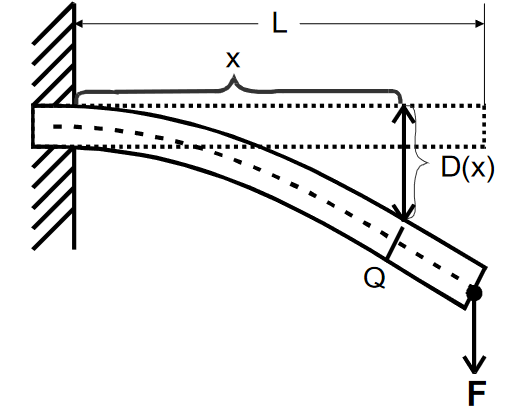
\includegraphics[width=7cm, keepaspectratio]{Biegung einseitig}
\caption{Biegung bei einseitiger Einspannung}
\label{fig:einseitig}
\end{figure}
Dieses führt dazu, dass die oberen Schichten des Stabes gestreckt und die unteren gestaucht werden, während in der Mitte eine neutrale Faser existiert,
welche nicht verformt wird. Aus dieser Streckung bzw. Stauchung resultieren Schubspannungen oberhalb und Druckspannungen unterhalb der neutralen Faser.
Die von ihnen verursachten Drehmomente sind entgegengesetzt gleich und lassen sich durch Integration über die Gesamte Querschnittsfläche $Q$ gemäß
\begin{equation*}
M_{\sigma}=\int_{Q} y\sigma (y) dy
\end{equation*}
berechnen. Das innere Drehmoment der Spannungen wirkt dem äußeren entgegen, bis sie sich ausgleichen. Daher lässt sich aus $M_F=M_{\sigma}$ die Durchbiegung 
$D(x)$ bestimmen:
\begin{equation}
D(x)=\frac{F}{2EI}(Lx^2-\frac{x^3}{3})
\end{equation}
Wobei mit $I$ das Flächenträgheitsmoment bezeichnet wird. \\
\subsection{Durchbiegung bei beidseitiger Einspannung}
Neben der soeben diskutierten einseitigen Einspannung, kann das Elastizitätsmodul auch bestimmt werden, indem der Stab beidseitig eingespannt wird und eine Kraft
in der Mitte angreift, wie es in Abbildung \ref{fig:beidseitig} dargestellt ist. Auch in diesem Fall wirkt ein äußeres Drehmoment. Dieses beträgt für die eine hälfte des Stabes ($0\leq x \leq L/2$)
\begin{equation*}
M_F=-\frac{F}{2}x
\end{equation*}
\begin{figure}
\centering
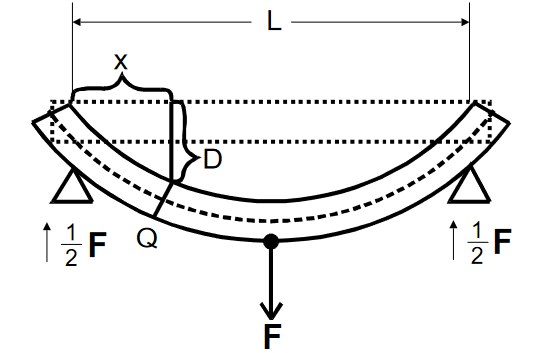
\includegraphics[width=7cm, keepaspectratio]{Biegung beidseitig}
\caption{Biegung bei beidseitiger Einspannung}
\label{fig:beidseitig}
\end{figure}
und dementsprechend für die andere hälfte ($L/2\leq x \leq L$)
\begin{equation*}
M_F=-\frac{F}{2}(L-x).
\end{equation*}
Daraus lässt sich mit einer Rechnung analog zu der vorherigen erneut die Durchbiegung in Abhängigkeit vom Abstand bestimmen. Diese beträgt
\begin{equation}
D(x)=\frac{F}{48EI}(3L^2x-4x^3)
\end{equation}
für den Bereich $0\leq x \leq L/2$ und 
\begin{equation}
D(x)=\frac{F}{48EI}(4x^3-12Lx^2+9L^2x-L^3)
\end{equation}
im anderen Bereich $L/2\leq x \leq L$.
